\documentclass[11pt,reqno]{amsart}

\usepackage[T1]{fontenc}
\usepackage[utf8]{inputenc}
\usepackage{mathpazo}
\usepackage{amsmath,amssymb,amsthm}
\usepackage{booktabs}
\usepackage{microtype}
\usepackage[margin=1.15in]{geometry}
\usepackage{tikz}
\usetikzlibrary{arrows.meta,positioning,decorations.pathreplacing}
\usepackage[colorlinks=true,linkcolor=blue!55!black,citecolor=blue!55!black,
            urlcolor=blue!55!black,hypertexnames=false,
            pdftitle={Full entropy dimension for a countable strongly
                      overlapping 3-adic renewal measure},
            pdfauthor={Eric Grover},
            pdfsubject={Mathematics (28A80, 11K41, 37A44, 94A17)},
            pdfkeywords={self-similar measure, overlaps, p-adic,
                         entropy dimension, renewal process}]{hyperref}

\theoremstyle{plain}
\newtheorem{theorem}{Theorem}[section]
\newtheorem{proposition}[theorem]{Proposition}
\newtheorem{lemma}[theorem]{Lemma}
\newtheorem{corollary}[theorem]{Corollary}
\theoremstyle{definition}
\newtheorem{definition}[theorem]{Definition}
\newtheorem{conjecture}[theorem]{Conjecture}
\theoremstyle{remark}
\newtheorem{remark}[theorem]{Remark}

\newcommand{\Zp}{\mathbb{Z}_p}
\newcommand{\Zthree}{\mathbb{Z}_3}
\newcommand{\Col}{\operatorname{Col}}
\newcommand{\E}{\mathbb{E}}
\newcommand{\Prob}{\operatorname{Pr}}
\DeclareMathOperator{\diment}{\underline{dim}_{\mathrm{ent}}}

\begin{document}

\title[Full entropy dimension for a $3$-adic renewal measure]
      {Full entropy dimension for a countable\\ strongly overlapping
       $3$-adic renewal measure}

\author{Eric Grover}
\address{Independent researcher}
\email{\href{mailto:eric@ericgrover.com}{eric@ericgrover.com}}

\subjclass[2020]{Primary 28A80; Secondary 11K41, 37A44, 94A17}
\keywords{self-similar measure, iterated function system with overlaps,
$p$-adic dynamics, entropy dimension, renewal process, collision entropy}

\begin{abstract}
Let $K_0,K_1,\ldots$ be independent with $\Prob(K=k)=2^{-k}$, $k\ge1$, put
$S_j=K_0+\cdots+K_j$, and let $\nu$ be the law of
\[
X=\sum_{j\ge0}3^j2^{-S_j}\in\Zthree .
\]
Equivalently $\nu$ is the stationary measure of the countably infinite
iterated function system $\phi_k(x)=(1+3x)/2^k$ with weights $2^{-k}$,
whose images overlap heavily. We prove that the level-$n$ collision number
$R_n=3^n\sum_c\Prob(X\equiv c)^2$ satisfies $R_n\le82n^3$, hence that the
entropy deficit is $O(\log n)$ and $\nu$ has full entropy dimension in
$\Zthree$. The proof is elementary: at a fixed renewal total, distinct
words in one $3$-adic cylinder are separated on the real line, and
decomposing simultaneously by renewal total and by dyadic real scale
converts that separation into an $L^2$ estimate whose two aggregate charges
are bounded by $1$ and $n/6$.

We then show the method is rigid. Within the natural family indexed by
coprime $p,q\ge2$ and a geometric gap parameter $\lambda$, the three
hypotheses the proof requires hold simultaneously for exactly one triple,
namely $(p,q,\lambda)=(3,2,1/2)$, and all three hold with equality.
We stress that the method delivers a polynomial of degree three whereas
machine-precision computation of $R_n$ to level $14$, from the exact
recurrence, indicates the truth is degree one.
We isolate the two independent factors of $n$ responsible, record the two
statements that would close the gap, and identify the structural reason
neither is reachable here: the stationary real address has critical moment
exponent exactly $1$, so it possesses no moment of order $\ge1$, and every
geometric weighting of the scale decomposition is therefore unavailable.
\end{abstract}

\maketitle

\section{Introduction}

\subsection{The measure}
All logarithms are natural. Let $K$ have the geometric law
\begin{equation}
\Prob(K=k)=2^{-k},\qquad k=1,2,\ldots,
\label{eq:gaplaw}
\end{equation}
let $K_0,K_1,\ldots$ be independent copies of $K$, and set
$S_j=K_0+\cdots+K_j$. The $j$-th term of
\begin{equation}
X=\sum_{j\ge0}3^j2^{-S_j}
\label{eq:X}
\end{equation}
has $3$-adic valuation $j$, so the series converges in $\Zthree$. Write
$\nu$ for its law. Since $X\equiv2^{-K_0}\not\equiv0\pmod3$, the measure
$\nu$ is supported on $\Zthree^\times$.

Equivalently, $\nu$ is the unique stationary measure of the iterated
function system
\begin{equation}
\phi_k(x)=\frac{1+3x}{2^k},\qquad \Prob(\phi_k)=2^{-k},\qquad k\ge1 .
\label{eq:ifs}
\end{equation}
Every map contracts by exactly $1/3$ in the $3$-adic metric, so the
similarity dimension is $h/\log3$ with $h=H(K)=2\log2$, giving
$2\log2/\log3\approx1.26>1$. The system is therefore supercritical, and the
question is whether the overlaps destroy entropy. Two features place it
outside the existing theory: the alphabet is countably infinite, and the
overlaps are severe, since $\phi_k$ and $\phi_{k'}$ have images meeting in
sets of full relative measure.

For $n\ge1$ only the first $n$ terms of \eqref{eq:X} affect the residue
modulo $3^n$. Put
\begin{equation}
C_n=\sum_{j=0}^{n-1}3^j2^{-S_j}\bmod 3^n,
\qquad p_n(c)=\Prob(C_n=c),
\label{eq:Cn}
\end{equation}
and define the collision number and the entropy deficit
\begin{equation}
R_n=3^n\sum_{c\bmod 3^n}p_n(c)^2,
\qquad
D_n=n\log3-H(C_n).
\label{eq:RnDn}
\end{equation}

\subsection{Results}

\begin{theorem}\label{thm:main}
For every $n\ge1$,
\begin{equation}
R_n\le70n^2\Bigl(1+\frac n6\Bigr)+2\gamma^n,
\qquad \gamma=\frac{3^{13}}{5^{10}}<1 .
\label{eq:mainbound}
\end{equation}
In particular $R_n\le82n^3$ and
\begin{equation}
D_n\le\log82+3\log n=o(n),
\label{eq:deficit}
\end{equation}
so that $H(C_n)/(n\log3)\to1$: the measure $\nu$ has full entropy dimension
in $\Zthree$.
\end{theorem}

Sections \ref{sec:words}--\ref{sec:proof} prove Theorem~\ref{thm:main}.
Section~\ref{sec:rigidity} proves that the method reaches exactly one
system, Section~\ref{sec:trueorder} quantifies how far $O(n^3)$ is from the
truth, and Section~\ref{sec:corollary} records an equivalent
affine-correlation form.

\subsection{Relation to the literature}
The entropy and dimension theory of overlapping self-similar measures on
$\mathbb R$ is by now substantial, but it does not cover the present
system, for two independent reasons.

First, \emph{finiteness}. Hochman's inverse entropy theorem \cite{Hochman14}
and its descendants---Shmerkin's $L^q$ formula under exponential separation
\cite{Shmerkin19}, Varj\'u's results for transcendental and algebraic
parameters \cite{Varju19ann,Varju19jams}, Breuillard--Varj\'u
\cite{BV19,BV20}, Rapaport \cite{Rapaport}---are all stated for a
\emph{finite} iterated function system; the recent survey \cite{Varju25}
defines an IFS as a finite collection in its opening sentence. Countable
conformal systems do have a dimension theory, due to Mauldin and Urba\'nski
\cite{MU96}, but it assumes the open set condition. With overlaps and a
countable alphabet one has pressure and overlap-function estimates
\cite{MihUrb13,MihUrb16}, not an identification with the similarity
dimension.

Second, \emph{effectivity}. Even where the real-line theory applies, it is
not quantitative. Hochman remarks explicitly, immediately after his
inverse theorem, that although the dependence of $\delta$ on $(\varepsilon,m)$
is effective, ``the value of $n$ depends among other things on the rate at
which $H_m(\mu)\to\dim\mu$, which is currently not effective''
\cite[\S2]{Hochman14}. Consequently no bound of the shape ``entropy deficit
at scale $n$ is at most $f(n)$'' with explicit $f$ follows from that theory.
Theorem~\ref{thm:main} is of exactly that shape, with every constant
written down.

In the $p$-adic setting, Hare and V\'avra \cite{HareVavra24} develop
self-similar sets and measures in $\mathbb Q_p$, but for a \emph{finite}
system whose contraction ratios are integer powers of $p$ and whose
translations are rational; their theory is of finite type and
automata-theoretic, and their open questions do not concern overlaps in the
present sense. Earlier $p$-adic constructions \cite{AbramLagarias14} are
graph-directed and separated. To the author's knowledge no ultrametric
analogue of the inverse entropy theorem exists. The entropy technology has
been transported to $\mathbb Q_p$ for the discretized sum-product problem
\cite{SalehiGolsefidy}, but not to self-similar measures.

The measure \eqref{eq:X} arose in an unrelated investigation and is studied
here on its own terms; nothing below bears on that origin.

\subsection{Acknowledgements}
The numerical work reported in Section~\ref{sec:trueorder} and the
verification scripts described in Appendix~\ref{app:anc} were carried out
with computational assistance. All statements labelled as theorems, lemmas
or propositions are proved in full in the text and do not depend on any
computation.

\section{Finite renewal words and real separation}\label{sec:words}

Let $w=(k_0,\ldots,k_{n-1})\in\mathbb Z_{\ge1}^n$ be a renewal word. Put
\begin{equation}
s_j(w)=k_0+\cdots+k_j,\qquad t(w)=s_{n-1}(w),
\label{eq:partials}
\end{equation}
and define the \emph{finite address}
\begin{equation}
x_n(w)=\sum_{j=0}^{n-1}3^j2^{-s_j(w)}=\frac{N_n(w)}{2^{t(w)}},
\qquad
N_n(w)=\sum_{j=0}^{n-1}3^j2^{t(w)-s_j(w)}\in\mathbb Z .
\label{eq:address}
\end{equation}
Note that $x_n(w)$ is simultaneously a positive rational number and, since
$2$ is a unit in $\Zthree$, an element of $\Zthree$ reducing to the cylinder
address of $w$. This double reading is the engine of the whole argument.
The probability of $w$ is
\begin{equation}
\Prob(w)=\prod_{j=0}^{n-1}2^{-k_j}=2^{-t(w)} ,
\label{eq:wordprob}
\end{equation}
which depends on $w$ only through its total.

\begin{lemma}[Word recovery]\label{lem:recovery}
The pair $(N_n(w),t(w))$ determines $w$ uniquely. In particular distinct
words of the same total have distinct addresses.
\end{lemma}

\begin{proof}
For $n=1$ we have $N_1(w)=1$ identically and $t(w)=k_0$, so $t$ alone
determines $w$. Let $n\ge2$. In \eqref{eq:address} the summand $j=n-1$
equals $3^{n-1}$, which is odd, while every summand with $j<n-1$ has
exponent $t-s_j\ge k_{n-1}\ge1$ and is even; hence $N_n(w)$ is odd.
Moreover
\[
N_n(w)-3^{n-1}=\sum_{j=0}^{n-2}3^j2^{t-s_j},
\]
and every exponent here is at least $k_{n-1}$. Factoring out
$2^{k_{n-1}}$ and using $t-k_{n-1}=s_{n-2}$ leaves
$\sum_{j\le n-2}3^j2^{s_{n-2}-s_j}$, whose $j=n-2$ term is the odd number
$3^{n-2}$ and whose earlier terms are even. Therefore
\begin{equation}
k_{n-1}=v_2\bigl(N_n(w)-3^{n-1}\bigr),
\label{eq:decode}
\end{equation}
and the quotient $(N_n(w)-3^{n-1})/2^{k_{n-1}}$ is precisely the numerator
attached to the prefix $(k_0,\ldots,k_{n-2})$, whose total is
$t-k_{n-1}$. Induction recovers every increment.
\end{proof}

\begin{lemma}[Fixed-total cylinder separation]\label{lem:separation}
Let $u\ne v$ be words of length $n$ with the same total $t$. If
$x_n(u)\equiv x_n(v)\pmod{3^n}$ then
\begin{equation}
|x_n(u)-x_n(v)|\ \ge\ \frac{2\cdot3^n}{2^t}\ =:\ \Delta_{n,t}.
\label{eq:sep}
\end{equation}
\end{lemma}

\begin{proof}
The common denominator $2^t$ is a unit modulo $3^n$, so the hypothesis
gives $3^n\mid N_n(u)-N_n(v)$. By Lemma~\ref{lem:recovery} that difference
is nonzero, and by the proof of Lemma~\ref{lem:recovery} both numerators
are odd, so the difference is even. As $\gcd(2,3^n)=1$ we get
$|N_n(u)-N_n(v)|\ge2\cdot3^n$, and division by $2^t$ gives \eqref{eq:sep}.
\end{proof}

Finally, since $s_j(w)\ge j+1$,
\begin{equation}
0<x_n(w)\le\sum_{j=0}^{n-1}\frac{3^j}{2^{j+1}}=\Bigl(\frac32\Bigr)^n-1 .
\label{eq:sizebound}
\end{equation}

\begin{figure}[t]
\centering
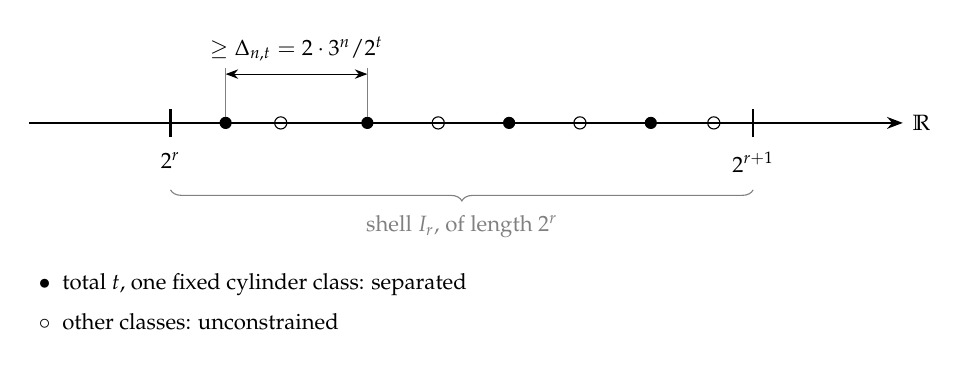
\begin{tikzpicture}[x=1cm,y=1cm]
\draw[-{Stealth[length=2mm]},thick] (-0.2,0) -- (10.9,0);
\node[right] at (10.9,0) {\footnotesize $\mathbb R$};
\draw[thick] (1.6,-0.18) -- (1.6,0.18);
\node[below=2pt] at (1.6,-0.18) {\footnotesize $2^r$};
\draw[thick] (9.0,-0.18) -- (9.0,0.18);
\node[below=2pt] at (9.0,-0.18) {\footnotesize $2^{r+1}$};
\foreach \x in {2.3,4.1,5.9,7.7}{\fill (\x,0) circle (2.2pt);}
\foreach \x in {3.0,5.0,6.8,8.5}{\draw[thin] (\x,0) circle (2.2pt);}
\draw[{Stealth[length=1.6mm]}-{Stealth[length=1.6mm]},thin] (2.3,0.62) -- (4.1,0.62);
\draw[thin,gray] (2.3,0.08) -- (2.3,0.7);
\draw[thin,gray] (4.1,0.08) -- (4.1,0.7);
\node[above=1pt] at (3.2,0.62)
   {\footnotesize $\ge\Delta_{n,t}=2\cdot3^n/2^t$};
\draw[decorate,decoration={brace,amplitude=4pt,mirror},gray]
  (1.6,-0.85) -- (9.0,-0.85);
\node[gray] at (5.3,-1.32) {\footnotesize shell $I_r$, of length $2^r$};
\node[anchor=west] at (-0.2,-2.05)
 {\footnotesize $\bullet$\; total $t$, one fixed cylinder class: separated};
\node[anchor=west] at (-0.2,-2.52)
 {\footnotesize $\circ$\; other classes: unconstrained};
\end{tikzpicture}
\caption{Lemma~\ref{lem:separation}. Within one $3$-adic cylinder and one
renewal total, real addresses are $\Delta_{n,t}$-separated, so a dyadic
shell of length $2^r$ carries at most $1+2^r/\Delta_{n,t}$ of them.
Addresses in different classes are subject to no such constraint.}
\label{fig:sep}
\end{figure}

\section{Decomposition by total and by real scale}\label{sec:decomp}

Fix $n$. For an integer $t\ge n$ and $r\in\mathbb Z$ let
$I_r=[2^r,2^{r+1})$ and define the subprobability on $\mathbb Z/3^n\mathbb Z$
\begin{equation}
p_{t,r}(c)=\sum_{\substack{w\in\mathbb Z_{\ge1}^n:\ t(w)=t\\
x_n(w)\in I_r,\ x_n(w)\equiv c\ (3^n)}}2^{-t},
\qquad
\varepsilon_{t,r}=\|p_{t,r}\|_1 .
\label{eq:cells}
\end{equation}
We refer to the pairs $(t,r)$ as \emph{cells}.

\begin{lemma}[Cell atom bound]\label{lem:atom}
For every cell,
\begin{equation}
\|p_{t,r}\|_\infty\le2^{-t}+\frac{2^r}{2\cdot3^n},
\qquad\text{hence}\qquad
3^n\|p_{t,r}\|_2^2\le\bigl(3^n2^{-t}+2^{r-1}\bigr)\varepsilon_{t,r}.
\label{eq:atom}
\end{equation}
\end{lemma}

\begin{proof}
By Lemma~\ref{lem:separation} the addresses of a fixed total lying in one
residue class are mutually separated by at least $\Delta_{n,t}$, so the
interval $I_r$, of length $2^r$, contains at most $1+2^r/\Delta_{n,t}$ of
them. Each carries weight $2^{-t}$ by \eqref{eq:wordprob}, which is the
first claim. The second follows from
$\sum_cp_{t,r}(c)^2\le\|p_{t,r}\|_\infty\|p_{t,r}\|_1$.
\end{proof}

We retain all totals in the range
\begin{equation}
n\le t<6n,
\label{eq:core}
\end{equation}
which we call the \emph{core}; there is no lower-tail deletion. If $t<6n$
then $x_n(w)\ge2^{-k_0}\ge2^{-t}>2^{-6n}$, since $k_0\le t$. Together with
\eqref{eq:sizebound} this confines core addresses to shells with
\begin{equation}
-6n\le r<n .
\label{eq:shellrange}
\end{equation}
There are at most $7n$ such shells and exactly $5n$ totals in
\eqref{eq:core}, so the number $Q_n$ of nonempty core cells obeys
\begin{equation}
Q_n\le35n^2 .
\label{eq:Qn}
\end{equation}

\begin{remark}\label{rem:Qsharp}
Inequality \eqref{eq:shellrange} is slightly generous: \eqref{eq:sizebound}
gives $r\le\lfloor n\log_2(3/2)\rfloor$, so the exact count of admissible
cells is
\[
Q_n\le5n\bigl(6n+\lfloor n\log_2(3/2)\rfloor+1\bigr)
\le 32.925\,n^2+5n .
\]
This is asymptotically $32.93n^2$, but it is \emph{not} bounded by $33n^2$
for small $n$: at $n=1,2,3,4,6,\dots$ the left side exceeds $33n^2$, and it
equals $35n^2$ exactly at $n=1$ and $n=2$. The clean bound
\eqref{eq:Qn} is therefore the one to use. What equals $35n^2$ at $n=1,2$
is the rectangular range count above, not the number $Q_n$ of nonempty
cells, which is far smaller ($Q_1=5$, $Q_2=46$; see
Section~\ref{sec:trueorder});
replacing it by the asymptotic form would gain nothing in
Theorem~\ref{thm:main}, whose constant is determined entirely by $n=1$.
\end{remark}

\section{The two aggregate charges}\label{sec:charges}

The point of the decomposition is that the two terms of \eqref{eq:atom}
aggregate over all cells with no loss exponential in $n$.

\begin{lemma}[Diagonal charge]\label{lem:diag}
$\displaystyle 3^n\sum_{t,r}2^{-t}\varepsilon_{t,r}\le1$, the sum being over
core cells.
\end{lemma}

\begin{proof}
The total $T_n=S_{n-1}$ is negative binomial,
$\Prob(T_n=t)=\binom{t-1}{n-1}2^{-t}$ for $t\ge n$, and the shells
partition the words of a fixed total, so $\sum_r\varepsilon_{t,r}\le\Prob(T_n=t)$.
Hence
\[
3^n\sum_{t,r}2^{-t}\varepsilon_{t,r}
\le3^n\sum_{t\ge n}\binom{t-1}{n-1}4^{-t}
=3^n\Bigl(\frac{1/4}{1-1/4}\Bigr)^n=3^n3^{-n}=1,
\]
using $\sum_{t\ge n}\binom{t-1}{n-1}z^t=(z/(1-z))^n$ at $z=1/4$.
\end{proof}

\begin{lemma}[Shell charge]\label{lem:shell}
$\displaystyle \sum_{t,r}2^{r-1}\varepsilon_{t,r}\le\frac n6$.
\end{lemma}

\begin{proof}
On $I_r$ one has $2^r\le x_n(w)$, so
$\sum_{t,r}2^{r-1}\varepsilon_{t,r}\le\tfrac12\E[x_n(W)]$. Now
$\E[2^{-K}]=\sum_{k\ge1}4^{-k}=1/3$, so by independence
$\E[2^{-S_j}]=3^{-(j+1)}$ and
\begin{equation}
\E[x_n(W)]=\sum_{j=0}^{n-1}3^j\cdot3^{-(j+1)}=\frac n3 .
\label{eq:firstmoment}
\end{equation}
\end{proof}

\begin{remark}[The crux]\label{rem:crux}
Identity \eqref{eq:firstmoment} is the whole theorem, and it is worth
isolating why. The address has \emph{exponential range} but \emph{linear
mean}: $x_n$ may be as large as $(3/2)^n-1$ by \eqref{eq:sizebound}, yet
$\E[x_n]=n/3$ because each term contributes exactly
$3^j\cdot3^{-(j+1)}=1/3$. High shells therefore carry exponentially little
mass, which is precisely what defeats the exponentially large factor
$2^{r-1}$ in \eqref{eq:atom}. An argument using only the sup bound
\eqref{eq:sizebound} in place of the first moment yields nothing: it
produces the factor $2^{r-1}\le2^{0.585n}$ in every cell. This exact
balance is also what fails for every other parameter choice, as
Section~\ref{sec:rigidity} shows.
\end{remark}

\begin{proposition}[Core collision bound]\label{prop:core}
Let $p_n^{\mathrm{core}}$ be the subprobability contributed by the totals
$n\le T_n<6n$ and $R_n^{\mathrm{core}}=3^n\|p_n^{\mathrm{core}}\|_2^2$. Then
\begin{equation}
R_n^{\mathrm{core}}\le35n^2\Bigl(1+\frac n6\Bigr).
\label{eq:corebound}
\end{equation}
\end{proposition}

\begin{proof}
By Lemma~\ref{lem:atom} and Lemmas~\ref{lem:diag}, \ref{lem:shell},
\begin{equation}
\sum_{t,r}3^n\|p_{t,r}\|_2^2\le1+\frac n6 .
\label{eq:sumsq}
\end{equation}
Writing $a_{t,r}=3^{n/2}\|p_{t,r}\|_2$, Minkowski's inequality and then
Cauchy--Schwarz over the at most $Q_n$ nonempty cells give
\[
\sqrt{R_n^{\mathrm{core}}}
=3^{n/2}\Bigl\|\sum_{t,r}p_{t,r}\Bigr\|_2
\le\sum_{t,r}a_{t,r}
\le\Bigl(Q_n\sum_{t,r}a_{t,r}^2\Bigr)^{1/2}.
\]
Now apply \eqref{eq:Qn} and \eqref{eq:sumsq} and square.
\end{proof}

\section{Upper tail and proof of Theorem~\ref{thm:main}}\label{sec:proof}

Since $\E[z^K]=z/(2-z)$ for $0<z<2$, exponential Markov at $z=5/3$ gives
\begin{equation}
\Prob(T_n\ge6n)\le z^{-6n}\Bigl(\frac z{2-z}\Bigr)^n
=\Bigl[\Bigl(\tfrac35\Bigr)^6\cdot5\Bigr]^n
=\Bigl(\frac{729}{3125}\Bigr)^n .
\label{eq:chernoff}
\end{equation}
Writing $p_n^{\mathrm{tail}}$ for the subprobability from $T_n\ge6n$ and
using $\|p\|_2^2\le\|p\|_1^2$,
\begin{equation}
R_n^{\mathrm{tail}}\le3^n\Prob(T_n\ge6n)^2
\le\Bigl[3\Bigl(\tfrac{729}{3125}\Bigr)^2\Bigr]^n=\gamma^n,
\qquad
\gamma=\frac{1594323}{9765625}=\frac{3^{13}}{5^{10}} .
\label{eq:tail}
\end{equation}
Numerically $\gamma\approx0.16325868<1$. (Any $z\in(1,2)$ works in
\eqref{eq:chernoff}; $z=5/3$ is chosen for arithmetic convenience.)

Since $p_n=p_n^{\mathrm{core}}+p_n^{\mathrm{tail}}$, the $L^2$ triangle
inequality and $(a+b)^2\le2a^2+2b^2$ give
\[
R_n\le2R_n^{\mathrm{core}}+2R_n^{\mathrm{tail}}
\le70n^2\Bigl(1+\frac n6\Bigr)+2\gamma^n,
\]
which is \eqref{eq:mainbound}. For the cubic form, divide by $n^3$:
\[
\frac{70n^2\bigl(1+n/6\bigr)+2\gamma^n}{n^3}
=\frac{35}3+\frac{70}n+\frac{2\gamma^n}{n^3}.
\]
Each of the last two terms is strictly decreasing in $n\ge1$, so the right
side attains its maximum at $n=1$, where it equals
\[
\frac{245}3+2\gamma<\frac{245}3+\frac13=82,
\]
since $\gamma=3^{13}/5^{10}<1/6$. Hence $R_n\le82n^3$ for every $n\ge1$,
which is \eqref{eq:deficit}'s hypothesis.
Finally, Shannon entropy dominates order-two R\'enyi entropy, so
$H(C_n)\ge-\log\sum_cp_n(c)^2=n\log3-\log R_n$, whence $D_n\le\log R_n$ and
\eqref{eq:deficit} follows. Dividing by $n\log3$ gives full entropy
dimension. \qed

\section{Rigidity of the method}\label{sec:rigidity}

It is natural to ask whether Theorem~\ref{thm:main} is one member of a
family. It is not. We show that the hypotheses the proof needs single out
the triple $(3,2,1/2)$, and that all of them hold with equality there.

Fix coprime integers $p,q\ge2$ and $\lambda\in(0,1)$, let the gaps be
geometric,
\begin{equation}
w_k=\Prob(K=k)=(1-\lambda)\lambda^{k-1},\qquad k\ge1,
\label{eq:geomgap}
\end{equation}
and consider $X=\sum_{j\ge0}p^jq^{-S_j}\in\Zp$, with finite addresses
$x_n(w)=\sum_{j<n}p^jq^{-s_j}=N_n(w)/q^{t}$ as in \eqref{eq:address}.
Lemma~\ref{lem:recovery} goes through verbatim with $v_2$ replaced by
$v_q$, and since $N_n\equiv p^{n-1}\pmod q$ for every word of length $n$,
Lemma~\ref{lem:separation} becomes
$|x_n(u)-x_n(v)|\ge q\,p^n/q^{t}$. The word probability is
$\pi(t)=(1-\lambda)^n\lambda^{t-n}$, again a function of the total alone.
Three quantities then control the argument.

\begin{definition}\label{def:hyp}
With the notation above set
\[
\gamma_{\mathrm{d}}=p\sum_{k\ge1}w_k^2=\frac{p(1-\lambda)}{1+\lambda},
\qquad
\gamma_{\mathrm{m}}=p\,\E[q^{-K}]=\frac{p(1-\lambda)}{q-\lambda},
\qquad
\gamma_{\mathrm{s}}=\frac{(1-\lambda)^2q}{1-\lambda^2q},
\]
the last defined when $\lambda^2q<1$. The hypotheses are
\begin{equation}
\mathrm{(H1)}\ \gamma_{\mathrm{d}}\le1,
\qquad
\mathrm{(H2)}\ \gamma_{\mathrm{m}}\le1,
\qquad
\mathrm{(H3)}\ \gamma_{\mathrm{s}}\le1 .
\label{eq:H}
\end{equation}
\end{definition}

Their roles are as follows. \textup{(H1)} is Lemma~\ref{lem:diag}: the
diagonal charge equals $\bigl(p\sum_kw_k^2\bigr)^n$, so it is bounded
exactly when the collision entropy of the gap law is at least $\log p$.
\textup{(H2)} is Lemma~\ref{lem:shell}: $\E[x_n]=m\sum_{j<n}(pm)^j$ with
$m=\E[q^{-K}]$, which is linear in $n$ when $pm=1$, bounded when $pm<1$,
and exponential otherwise. \textup{(H3)} controls the shell prefactor. In
\eqref{eq:atom} the second term carries the factor $q^{t-1}\pi(t)$, which
is constant in $t$ only if $\lambda q=1$; in general, summing
$2^r\le x_n$ against the law of $T_n$ yields
\begin{equation}
\sum_{t,r}2^rq^{t-1}\pi(t)\varepsilon_{t,r}
\le\frac1q\cdot\frac{1-\lambda}{1+\lambda}
\sum_{j<n}\gamma_{\mathrm{s}}^{\,n-1-j}\gamma_{\mathrm{d}}^{\,j},
\label{eq:shellgeneral}
\end{equation}
which is polynomial in $n$ precisely when
$\gamma_{\mathrm{s}}\le1$ and $\gamma_{\mathrm{d}}\le1$.

\begin{theorem}[Rigidity]\label{thm:rigidity}
Let $p,q\ge2$ be coprime integers and $\lambda\in(0,1)$ with
$\lambda^2q<1$. Then \textup{(H1)}, \textup{(H2)} and \textup{(H3)} hold
simultaneously if and only if
\[
(p,q,\lambda)=\bigl(3,\,2,\,\tfrac12\bigr),
\]
and in that case
$\gamma_{\mathrm{d}}=\gamma_{\mathrm{m}}=\gamma_{\mathrm{s}}=1$.
\end{theorem}

\begin{proof}
Assume \textup{(H3)}. Since $\lambda^2q<1$, clearing the denominator gives
$(1-\lambda)^2q\le1-\lambda^2q$, that is
\begin{equation}
q\bigl[(1-\lambda)^2+\lambda^2\bigr]\le1 .
\label{eq:H3clean}
\end{equation}
The function $\lambda\mapsto(1-\lambda)^2+\lambda^2$ is strictly convex on
$(0,1)$ with minimum value $1/2$, attained only at $\lambda=1/2$. Hence
\eqref{eq:H3clean} forces $q/2\le1$, so $q=2$; and then equality
$2\cdot\frac12=1$ is required, so $\lambda=1/2$ and
$\gamma_{\mathrm{s}}=1$. Note $\lambda^2q=1/2<1$, consistent.

With $q=2$ and $\lambda=1/2$ we get
$\sum_kw_k^2=(1-\lambda)/(1+\lambda)=1/3$, so \textup{(H1)} reads
$p/3\le1$, i.e. $p\le3$. Since $p\ge2$ and $\gcd(p,2)=1$ we must have
$p=3$, and then $\gamma_{\mathrm{d}}=1$.

Finally $\E[q^{-K}]=(1-\lambda)/(q-\lambda)=\tfrac12/\tfrac32=1/3$, so
$\gamma_{\mathrm{m}}=3\cdot\tfrac13=1$ and \textup{(H2)} holds, again with
equality. Conversely $(3,2,1/2)$ satisfies all three, as just computed.
\end{proof}

\begin{remark}
The obstruction is \textup{(H3)}, and it is geometric rather than
arithmetic: separation is measured in a single archimedean absolute value,
and the resulting prefactor $q^{t-1}\pi(t)$ can be tamed only when the
geometric decay of the word probability exactly cancels the growth of
$q^{t}$. With $\lambda=1/q$, so that the gap law is $w_k=(q-1)q^{-k}$, the
prefactor equals $(q-1)^n/q$, bounded only for $q=2$. A route past this
barrier would presumably replace the single real place by a product formula
over several places; we do not pursue it.
\end{remark}

\begin{remark}
Theorem~\ref{thm:rigidity} explains why the measure \eqref{eq:X} is the one
that can be treated: it is the unique point at which the collision entropy
of the gap law, the first moment of the real address, and the shell
prefactor are all exactly critical. An exhaustive rational search over
coprime $p,q\le12$ and $\lambda=a/b$ with $b\le24$ returns this triple and
no other; see Appendix~\ref{app:anc}.
\end{remark}

\section{The true order of \texorpdfstring{$R_n$}{Rn}}\label{sec:trueorder}

Theorem~\ref{thm:main} is correct but not sharp. This section records what
is true, isolates the two independent losses, and states what would remove
them. Nothing here is used elsewhere in the paper.

Because $2$ is a primitive root modulo $3^n$, the recursion
$C_n\equiv2^{-K}(1+3C_{n-1})\pmod{3^n}$ is a cyclic convolution of length
$2\cdot3^{n-1}$ in discrete-logarithm coordinates, so $p_n$ and hence $R_n$
are computable to machine precision from that exact recurrence by fast
Fourier transform. (The finite-word computations reported later in this
section are, by contrast, exact integer arithmetic.) The result is

\begin{center}
\begin{tabular}{@{}rrrrr@{}}
\toprule
$n$ & $R_n$ & $R_n/n^3$ & $\mathcal G_n$ & $82n^3$\\
\midrule
$4$  & $3.06865$ & $0.04795$ & $0.23276$ & $5248$\\
$6$  & $4.00033$ & $0.01852$ & $0.23275$ & $17712$\\
$8$  & $4.93174$ & $0.00963$ & $0.23333$ & $41984$\\
$10$ & $5.86579$ & $0.00587$ & $0.23408$ & $82000$\\
$12$ & $6.80290$ & $0.00394$ & $0.23481$ & $141696$\\
$14$ & $7.74277$ & $0.00282$ & --- & $225008$\\
\bottomrule
\end{tabular}
\end{center}

\noindent
where $\mathcal G_n=(R_{n+1}-R_n)/2$. A least-squares fit over
$7\le n\le13$ gives $R_n\approx0.468n+1.19$ to three decimals, and the
increments $\mathcal G_n$ drift upward by about one percent over seven
levels. The evidence is therefore for

\begin{conjecture}\label{conj:linear}
$R_n=\Theta(n)$, and consequently $D_n\le\log n+O(1)$.
\end{conjecture}

The two powers of $n$ separating \eqref{eq:mainbound} from
Conjecture~\ref{conj:linear} are independent and can be located exactly.
Write $a_{t,r}=3^{n/2}\|p_{t,r}\|_2$ as in Proposition~\ref{prop:core} and
define the \emph{effective cell count}
\[
\mathcal Q_n^{\mathrm{eff}}
=\frac{R_n^{\mathrm{core}}}{\sum_{t,r}a_{t,r}^2},
\]
so that $R_n^{\mathrm{core}}=\mathcal Q_n^{\mathrm{eff}}\sum a_{t,r}^2$
tautologically, and
$\mathcal Q_n^{\mathrm{eff}}\le\bigl(\sum a_{t,r}\bigr)^2/\sum a_{t,r}^2
\le Q_n$ by Minkowski and Cauchy--Schwarz. Proposition~\ref{prop:core}
replaces $\mathcal Q_n^{\mathrm{eff}}$ by the crude $Q_n$. Exact rational computation over all words with $n\le t<6n$
gives

\begin{center}
\begin{tabular}{@{}rrrrrr@{}}
\toprule
$n$ & $Q_n$ & $35n^2$ & $\sum a_{t,r}^2$ & $1+n/6$ & $\mathcal Q_n^{\mathrm{eff}}$\\
\midrule
$1$ & $5$   & $35$   & $0.99902$ & $1.1667$ & $1.5865$\\
$2$ & $46$  & $140$  & $0.99999$ & $1.3333$ & $2.1251$\\
$3$ & $106$ & $315$  & $1.00012$ & $1.5000$ & $2.6004$\\
$4$ & $191$ & $560$  & $1.00426$ & $1.6667$ & $3.0548$\\
$5$ & $325$ & $875$  & $1.00965$ & $1.8333$ & $3.5002$\\
$6$ & $437$ & $1260$ & $1.01892$ & $2.0000$ & $3.9260$\\
$7$ & $596$ & $1715$ & $1.02995$ & $2.1667$ & $4.3359$\\
\bottomrule
\end{tabular}
\end{center}

Two things are visible. First, $\sum a_{t,r}^2$ is flat, near $1$, whereas
Proposition~\ref{prop:core} uses the bound $1+n/6$; the shell charge of
Lemma~\ref{lem:shell} is never approached, because \eqref{eq:atom} replaces
$\sum_c(\text{count}_c)^2$ by $\max_c(\text{count}_c)\cdot\sum_c\text{count}_c$
and almost every class contains a single word. Second,
$\mathcal Q_n^{\mathrm{eff}}$ grows linearly, at roughly $0.44n+1.2$,
whereas Cauchy--Schwarz charges $Q_n=\Theta(n^2)$; the mass concentrates on
totals within $O(\sqrt n)$ of $2n$ and on shells within $O(1)$ of
$r=-K_0$, so the overwhelming majority of the $35n^2$ cells are negligible.

Each observation, if proved, removes one factor of $n$:

\begin{conjecture}\label{conj:two}
$\sum_{t,r}3^n\|p_{t,r}\|_2^2=O(1)$, and
$\mathcal Q_n^{\mathrm{eff}}=O(n)$.
\end{conjecture}

Together they give Conjecture~\ref{conj:linear}. We record the obstacles we
met. Restricting the ranges of $t$ and $r$ to the $O(\sqrt n)$ and $O(1)$
windows that carry the mass leaves a complement of only polynomially small
probability, and the crude estimate $R^{\mathrm{tail}}\le3^n\|p\|_1^2$ used
in \eqref{eq:tail} requires exponentially small mass; both ranges must
therefore stay of length $\Theta(n)$, which forces $Q_n=\Theta(n^2)$.
Weighted Cauchy--Schwarz does not help either, and it is worth recording
exactly why, because the reason locates the obstruction. Split
\eqref{eq:atom} as $a_{t,r}\le b_{t,r}+c_{t,r}$ with
$b_{t,r}=(3^n2^{-t}\varepsilon_{t,r})^{1/2}$ and
$c_{t,r}=(2^{r-1}\varepsilon_{t,r})^{1/2}$. For the diagonal part one can
indeed do better than Proposition~\ref{prop:core}: the summand
\[
f_t=3^n2^{-t}\Prob(T_n=t)=\binom{t-1}{n-1}\Bigl(\frac34\Bigr)^n
\Bigl(\frac14\Bigr)^{t-n}
\]
appearing in Lemma~\ref{lem:diag} is itself a negative binomial probability
mass function with parameters $(n,3/4)$, of total mass $1$, mean $4n/3$ and
standard deviation $\tfrac23\sqrt n$. Concentration therefore gives
$\sum_t\sqrt{f_t}=O(n^{1/4})$, numerically $1.828\,n^{1/4}$, and
Cauchy--Schwarz over the at most $7n$ shells of a given total yields
\begin{equation}
\sum_{t,r}b_{t,r}\le\sqrt{7n}\sum_t\sqrt{f_t}=O\bigl(n^{3/4}\bigr),
\label{eq:diagsector}
\end{equation}
against the $O(n)$ that \eqref{eq:Qn} alone provides. But the diagonal part
is not the leading term. The same manoeuvre fails for the shell part,
because $h_t=\sum_r2^{r-1}\varepsilon_{t,r}\approx\tfrac12\E[x_n;T_n=t]$
does \emph{not} concentrate: under the $x_n$-weighted measure the $j$-th
term of \eqref{eq:X} contributes near $T_n\approx2n-\tfrac23j$, so the
weight is spread over the whole window $[4n/3,2n]$, of width $\Theta(n)$.
One is left with
$\sum_{t,r}c_{t,r}\le\sqrt{7n}\,(5n\cdot n/6)^{1/2}=\sqrt{35/6}\,n^{3/2}$,
whose square is $\tfrac{35}6n^3$: exactly the leading constant of
Proposition~\ref{prop:core}. The refinement thus gains nothing at all, not
even in the constant.

The shell sector splits further, and the split isolates the obstruction
completely. For $r<0$ a geometric weight \emph{is} available: since
$\varepsilon_{t,r}\le\Prob(x_n<2^{r+1})\le\Prob(K_0>-r-1)=2^{r+1}$ and also
$\varepsilon_{t,r}\le\Prob(T_n=t)$,
\begin{equation}
\sum_{r<0}c_{t,r}
\le\sqrt{\Prob(T_n=t)}\sum_{r<0}2^{(r-1)/2}
=\frac{1}{2-\sqrt2}\sqrt{\Prob(T_n=t)},
\label{eq:negshell}
\end{equation}
so $\sum_{t}\sum_{r<0}c_{t,r}\le(2-\sqrt2)^{-1}\sqrt{5n}=O(\sqrt n)$; in
the exact finite-word enumeration this sum is in fact bounded, converging
to about
$1.6$. The whole difficulty lies in $0\le r\le n\log_2(3/2)$.

There the natural remedy is again a geometric weight, and it is
unavailable for a structural reason. Cauchy--Schwarz with
$u_{t,r}=2^{-\theta r}$, $\theta>0$, gives
\[
\sum_{t,\,r\ge0}c_{t,r}
\le\Bigl(\tfrac12\E\bigl[x_n^{1+\theta}\bigr]\Bigr)^{1/2}
\Bigl(\tfrac{5n}{1-2^{-\theta}}\Bigr)^{1/2},
\]
so it requires a moment of order $1+\theta$. No such moment exists.

\begin{lemma}\label{lem:moment}
The increasing limit $x=\lim_nx_n=\sum_{j\ge0}3^j2^{-S_j}$ is finite almost
surely. Moreover $\E[x^p]<\infty$ for every $0<p<1$, and $\E[x^p]=\infty$
for every $p\ge1$.
\end{lemma}

\begin{proof}
\emph{Almost sure finiteness.} Since $\E K=\sum_{k\ge1}k2^{-k}=2$, the
strong law of large numbers gives $S_j/(j+1)\to2$ almost surely. Fix
$\varepsilon$ with $0<\varepsilon<2-\log_23$, which is possible because
$\log_23<2$. Almost surely there is a $j_0$ with
$S_j\ge(2-\varepsilon)(j+1)$ for all $j\ge j_0$, and then
\[
3^j2^{-S_j}\le3^j2^{-(2-\varepsilon)(j+1)}
=2^{-(2-\varepsilon)}\Bigl(\frac{3}{2^{\,2-\varepsilon}}\Bigr)^{j}.
\]
The ratio $3\cdot2^{-(2-\varepsilon)}$ is less than $1$ precisely because
$\varepsilon<2-\log_23$, so the series $\sum_j3^j2^{-S_j}$ is dominated by a
convergent geometric series beyond $j_0$ and therefore converges almost
surely. (Termwise decay alone would not suffice.)

\emph{Finiteness of the moments below $1$.}
Let $0<p<1$. Subadditivity of $t\mapsto t^p$ on $[0,\infty)$ gives
$x_n^p\le\sum_{j<n}\bigl(3^j2^{-S_j}\bigr)^p$, so by independence
\[
\E\bigl[x_n^p\bigr]
\le\sum_{j<n}3^{jp}\,\E\bigl[2^{-pK}\bigr]^{j+1}
=\E\bigl[2^{-pK}\bigr]\sum_{j<n}
\Bigl(3^p\,\E\bigl[2^{-pK}\bigr]\Bigr)^{j}.
\]
Since $\E[2^{-pK}]=\sum_{k\ge1}2^{-(1+p)k}=(2^{1+p}-1)^{-1}$, the ratio is
$3^p\E[2^{-pK}]<1$ exactly when
\begin{equation}
3^p+1<2^{\,p+1},
\label{eq:moment}
\end{equation}
which holds precisely for $p<1$, with equality at $p=1$. The geometric
series is then bounded uniformly in $n$, and monotone convergence gives
$\E[x^p]<\infty$.

\emph{Divergence of the moments from $1$ up.}
For $p\ge1$ a finite $p$-th moment would force $\E[x]\le(\E[x^p])^{1/p}
<\infty$ by Lyapunov. But $x\overset{d}{=}2^{-K}(1+3x)$ with $K$
independent of $x$, so a finite mean would satisfy
\[
\E x=\E\bigl[2^{-K}\bigr]\bigl(1+3\,\E x\bigr)
=\tfrac13+\E x,
\]
which is absurd. Hence $\E x=\infty$ and no moment of order $p\ge1$ is
finite.
\end{proof}

Thus $x$ has \emph{critical moment exponent} exactly $1$. We do not assert
a precise tail asymptotic; only the critical moment statement is used
below. The very criticality that produces $\E[x_n]=n/3$ in
Lemma~\ref{lem:shell} forbids every geometric shell weight. This is the
same phenomenon as the triple equality of Theorem~\ref{thm:rigidity},
appearing a fourth time.

Numerically $\sum b_{t,r}$, $\sum c_{t,r}$ and $\sum a_{t,r}$ grow like
$n^{0.45}$, $n^{1.12}$ and $n^{0.84}$ over $3\le n\le7$, so a bound of
order $n^{2}$ is presumably true; it is simply not reachable by weighting
this decomposition. It is Lemma~\ref{lem:shell} itself, and not the
aggregation step, that must be improved. Improving
\eqref{eq:atom} by capping the per-class count at the total number of words
in the cell never binds, since the required inequality $n3^n<2^{2r-1}$ fails
for $r\le0.585n$. A sharper route appears to need a bound on
$\sum_c(\text{count}_c)^2$ directly, which is the quantity being estimated.

\begin{remark}\label{rem:cap}
Identity \eqref{eq:recurrence} together with $\mathcal G_n\ge0$ shows that
$R_n$ is nondecreasing; the computations above suggest, but do not prove,
that $R_n\to\infty$. \emph{If} $R_n\to\infty$, then two consequences
follow. First, $D_n\le\log R_n$ cannot yield $\sup_nD_n<\infty$, so the
$L^2$ method is capped at $D_n=O(\log n)$, which Theorem~\ref{thm:main}
already attains up to the constant. Second, writing $Z_n$ for the density
of the level-$n$ discretisation against Haar measure, $R_n=\|Z_n\|_{L^2}^2$,
so $(Z_n)$ is unbounded in $L^2$ and $\nu$ has no $L^2$ density. Absolute
continuity with an $L\log L$ density would not be excluded, but neither
conclusion is reachable by sharpening the present argument.
\end{remark}

\section{An equivalent affine-correlation form}\label{sec:corollary}

For completeness we record a reformulation. Let $F(x)=4x+1$, so
$F^h(x)=4^hx+(4^h-1)/3$, and put
$\Gamma_n(h)=\sum_{y\bmod3^n}p_n(y)p_n(F^h(y))$.

\begin{lemma}\label{lem:recurrence}
With $\Col_n=\sum_cp_n(c)^2$ and
$\mathcal G_n=3^n\sum_{h\ge1}4^{-h}\Gamma_n(h)$,
\begin{equation}
\Col_{n+1}=\tfrac13\Col_n+\tfrac23\sum_{h\ge1}4^{-h}\Gamma_n(h),
\qquad\text{equivalently}\qquad
R_{n+1}-R_n=2\mathcal G_n .
\label{eq:recurrence}
\end{equation}
\end{lemma}

\begin{proof}
Write $X=2^{-K}(1+3Y)$ and $X'=2^{-K'}(1+3Y')$ with $Y,Y'$ independent
copies of $X$, and let $d=K-K'$, whose law is
$\Prob(d)=1/(3\cdot2^{|d|})$.

First, a parity constraint. Modulo $3$ we have $2\equiv-1$, so
$X\equiv(-1)^K$ and $X'\equiv(-1)^{K'}$. A collision $X\equiv X'\pmod
{3^{n+1}}$ therefore forces $K\equiv K'\pmod2$, that is, $d$ even. Odd $d$
contributes nothing.

Second, the reduction. If $d=0$ the condition becomes $Y\equiv Y'\pmod
{3^n}$, of probability $\Col_n$, and $\Prob(d=0)=\sum_k4^{-k}=1/3$. If
$d=2h$ with $h\ge1$, then $X\equiv X'$ modulo $3^{n+1}$ reads
$2^{-2h}(1+3Y)\equiv1+3Y'$, i.e. $1+3Y\equiv4^h(1+3Y')$, i.e.
\[
Y\equiv\frac{4^h-1}3+4^hY'=F^h(Y')\pmod{3^n},
\]
of probability $\Gamma_n(h)$. Each of the two signs $d=\pm2h$ has
probability $1/(3\cdot2^{2h})=\tfrac13 4^{-h}$, so together they contribute
$\tfrac23 4^{-h}\Gamma_n(h)$. Summing over $h\ge1$ and adding the $d=0$
term gives \eqref{eq:recurrence}.
\end{proof}

\begin{corollary}\label{cor:G}
For every $n\ge1$, $\ \mathcal G_n\le41(n+1)^3$, and hence for any cutoff
$J(n)\ge1$,
$3^n\sum_{1\le h\le J(n)}4^{-h}\Gamma_n(h)\le41(n+1)^3$.
\end{corollary}

\begin{proof}
$\mathcal G_n\le R_{n+1}/2\le82(n+1)^3/2$ by \eqref{eq:recurrence},
$R_n\ge0$ and Theorem~\ref{thm:main}. The second claim follows by
positivity.
\end{proof}

The numerics of Section~\ref{sec:trueorder} indicate
$\mathcal G_n=O(1)$, with $\mathcal G_n\approx0.235$; Corollary~\ref{cor:G}
is far from sharp, and is stated only because the recurrence
\eqref{eq:recurrence} makes $\mathcal G_n$ the natural quantity.

\section{What is and is not proved}\label{sec:limits}

The argument uses no fitted state, no numerical extrapolation, and no
lower-tail cutoff; every total $n\le T_n<6n$, including the typical window
$T_n\sim2n$, is handled by the shell decomposition, and only the
exponentially rare tail $T_n\ge6n$ is removed.

Proved: the polynomial collision bound $R_n=O(n^3)$; $D_n=O(\log n)$; full
entropy dimension of $\nu$; the affine-correlation bound of
Corollary~\ref{cor:G}; and the rigidity of the method,
Theorem~\ref{thm:rigidity}.

Not proved: $\sup_nD_n<\infty$; absolute continuity of $\nu$ with respect
to Haar measure; an $L\log L$ density; or $R_n=\Theta(n)$. Full entropy
dimension permits a slowly diverging deficit and is strictly weaker than
any of these.

Two further limitations of the method should be stated explicitly. Both are
\emph{conditional} on $R_n\to\infty$, which the computations of
Section~\ref{sec:trueorder} indicate but which this paper does not prove.
What \eqref{eq:recurrence} does prove, since $\mathcal G_n\ge0$, is that
$R_n$ is nondecreasing.

\emph{First, the method is capped at $D_n=O(\log n)$.} The only route from
$R_n$ to the entropy deficit is the R\'enyi bound $D_n\le\log R_n$ of
Section~\ref{sec:proof}. If $R_n\to\infty$ then $\log R_n\to\infty$, and no
sharpening of Theorem~\ref{thm:main} can yield $\sup_nD_n<\infty$. Even the
optimal form of the present argument, $R_n=\Theta(n)$ as in
Conjecture~\ref{conj:linear}, would give only $D_n\le\log n+O(1)$, which
Theorem~\ref{thm:main} already attains up to the constant and the factor
$3$. Bounded deficit, and hence absolute continuity by the standard
implication, requires a genuinely different mechanism. Note that this
limitation concerns the \emph{method} and is insensitive to how large the
truth of $R_n$ actually is, provided only that it diverges.

\emph{Second, conditionally, $\nu$ has no $L^2$ density.} Writing $Z_n$ for
the density of the level-$n$ discretisation of $\nu$ against Haar measure,
$R_n=\|Z_n\|_{L^2}^2$. If $R_n\to\infty$ then the martingale $(Z_n)$ is
unbounded in $L^2$ and $\nu$ admits no square-integrable density. This
would not exclude absolute continuity with an $L\log L$ density, a strictly
weaker conclusion. We emphasise that the absence of an $L^2$ density is
\emph{not} among the results proved here: it rests on the numerical
evidence for divergence recorded in Section~\ref{sec:trueorder}.

\appendix

\section{Ancillary files}\label{app:anc}

The directory \texttt{anc/} accompanying this article contains a single
self-contained verifier, \texttt{verify\_renewal\_entropy.py}, requiring
only Python 3.8 and NumPy. It

\begin{itemize}\itemsep2pt
\item computes $p_n$ to machine precision, from the exact recurrence, by
the discrete-logarithm convolution of
Section~\ref{sec:trueorder} and reproduces the table of $R_n$ for
$n\le14$, together with $D_n$ and $\mathcal G_n$;
\item verifies the recurrence \eqref{eq:recurrence} to machine precision
for $n\le9$;
\item enumerates all renewal words with $n\le t<6n$ for $n\le7$ in exact
integer arithmetic and checks Lemma~\ref{lem:atom} atom by atom,
Lemma~\ref{lem:diag}, Lemma~\ref{lem:shell}, \eqref{eq:Qn} and
Proposition~\ref{prop:core}, reproducing the second table of
Section~\ref{sec:trueorder};
\item performs the exhaustive rational search behind
Theorem~\ref{thm:rigidity} over coprime $p,q\le12$ and $\lambda=a/b$ with
$b\le24$.
\end{itemize}

No statement in Sections~\ref{sec:words}--\ref{sec:rigidity} depends on
these computations; they reproduce the constants and the tables.

\begin{thebibliography}{99}

\bibitem{AbramLagarias14}
W.~Abram and J.~C. Lagarias,
\emph{$p$-adic path set fractals and arithmetic},
J. Fractal Geom. \textbf{1} (2014), 45--81.

\bibitem{BV19}
E.~Breuillard and P.~P. Varj\'u,
\emph{On the dimension of Bernoulli convolutions},
Ann. Probab. \textbf{47} (2019), 2582--2617.

\bibitem{BV20}
E.~Breuillard and P.~P. Varj\'u,
\emph{Entropy of Bernoulli convolutions and uniform exponential growth for
linear groups},
J. Anal. Math. \textbf{140} (2020), 443--481.

\bibitem{HareVavra24}
K.~G. Hare and T.~V\'avra,
\emph{Self-similar sets and measures in the $p$-adics},
J. Fractal Geom. \textbf{11} (2024), no. 3/4, 247--287.

\bibitem{Hochman14}
M.~Hochman,
\emph{On self-similar sets with overlaps and inverse theorems for entropy},
Ann. of Math. (2) \textbf{180} (2014), 773--822.

\bibitem{MU96}
R.~D. Mauldin and M.~Urba\'nski,
\emph{Dimensions and measures in infinite iterated function systems},
Proc. London Math. Soc. (3) \textbf{73} (1996), 105--154.

\bibitem{MihUrb13}
E.~Mihailescu and M.~Urba\'nski,
\emph{Hausdorff dimension of the limit set of conformal iterated function
systems with overlaps},
Contemp. Math. \textbf{600} (2013), 273--290.

\bibitem{MihUrb16}
E.~Mihailescu and M.~Urba\'nski,
\emph{Random countable iterated function systems with overlaps and
applications},
Adv. Math. \textbf{298} (2016), 726--758.

\bibitem{Rapaport}
A.~Rapaport,
\emph{Proof of the exact overlaps conjecture for systems with algebraic
contractions},
preprint, arXiv:2001.01332.

\bibitem{SalehiGolsefidy}
A.~Salehi Golsefidy,
\emph{Sum-product phenomena: $p$-adic case},
J. Anal. Math. \textbf{142} (2020), 349--419.

\bibitem{Shmerkin19}
P.~Shmerkin,
\emph{On Furstenberg's intersection conjecture, self-similar measures, and
the $L^q$ norms of convolutions},
Ann. of Math. (2) \textbf{189} (2019), 319--391.

\bibitem{Varju19ann}
P.~P. Varj\'u,
\emph{On the dimension of Bernoulli convolutions for all transcendental
parameters},
Ann. of Math. (2) \textbf{189} (2019), 1001--1011.

\bibitem{Varju19jams}
P.~P. Varj\'u,
\emph{Absolute continuity of Bernoulli convolutions for algebraic
parameters},
J. Amer. Math. Soc. \textbf{32} (2019), 351--397.

\bibitem{Varju25}
P.~P. Varj\'u,
\emph{Entropy rates in the dimension theory of self-similar measures},
preprint, arXiv:2509.22042.

\end{thebibliography}

\end{document}
